\section{Autoencoder Non-linear Manifold PROMs}

\begin{table}
	\centering
	\begin{tabular}{ lll }
	\toprule
	Layer & Type & Output Size  \\
	\midrule
	1 & Convolution & 512 $\times$ 16 \\
    2 & Convolution & 256 $\times$ 32 \\
    3 & Convolution & 128 $\times$ 64 \\
    4 & Dense & $\numPrimModes$ \\
	\bottomrule
	\end{tabular}
	\caption{\label{tab:caeArch}Convolutional encoder dimensions. Decoder mirrors encoder with transpose convolutional layers.}
\end{table}

\begin{figure}
    \begin{minipage}{0.49\linewidth}
        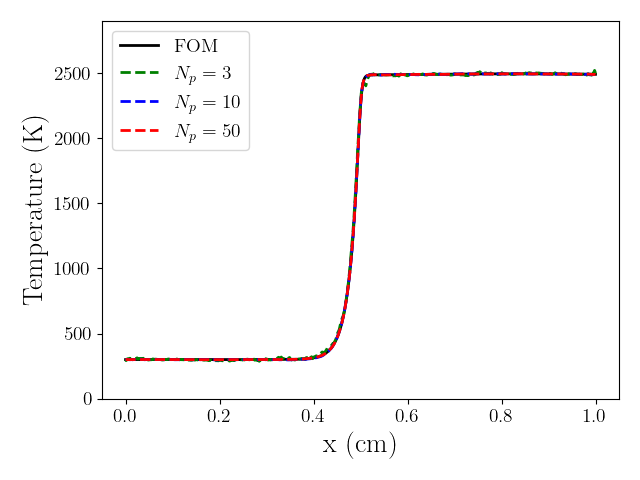
\includegraphics[width=0.99\linewidth]{Chapters/TransientFlame/Images/nonlinear/proj_temp_snaps.png}
    \end{minipage}
    \begin{minipage}{0.49\linewidth}
        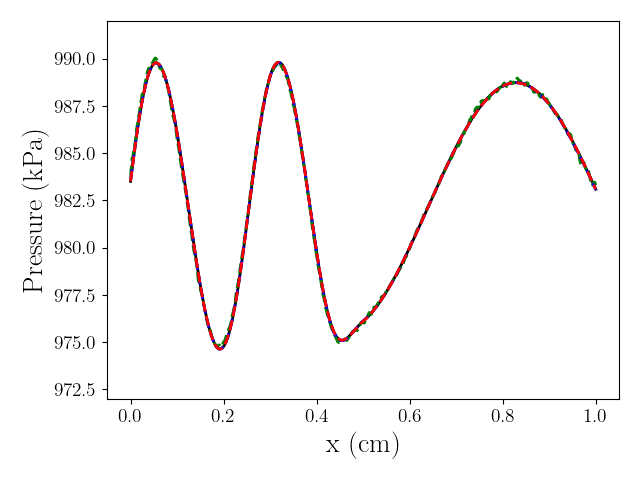
\includegraphics[width=0.99\linewidth]{Chapters/TransientFlame/Images/nonlinear/proj_press_snaps.png}
    \end{minipage}
    \caption{Approximation of temperature (left) and pressure (right) fields on solution manifold, $f = 150$ kHz, $\timeVar = 250 \mu$s, various $\numPrimModes$.}
\end{figure}

\begin{figure}
    \begin{minipage}{0.49\linewidth}
        \includegraphics[width=0.99\linewidth]{example-image-a}
    \end{minipage}
    \begin{minipage}{0.49\linewidth}
        \includegraphics[width=0.99\linewidth]{example-image-a}
    \end{minipage}
    \caption{Intrusive non-linear manifold MP-LSVT PROM snapshots, $\numPrimModes = XXX$.}
\end{figure}

\begin{table}
	\centering
	\begin{tabular}{ lll }
	\toprule
	Model & Runtime (hours) & Cost (FOM runs)  \\
	\midrule
    Online FOM ($\times 1$) & 0.42 & 1 \\
    Training, $\numPrimModes = 3$ & 5.8 & 13.81 \\
    Training, $\numPrimModes = 10$ & 4.9 & 11.67 \\
    Training, $\numPrimModes = 50$ & 5.5 & 13.1 \\
    Online NLM PROM, $\numPrimModes = 3$ & 7.2 & 17.14 \\
	\bottomrule
	\end{tabular}
	\caption{\label{tab:caeCost}Relative offline/online computational costs for NLM PROMs. Non-increasing CAE training costs are due to early stopping.}
\end{table}

\section{Recurrent Neural Network ROMs}

\begin{figure}
    \centering
    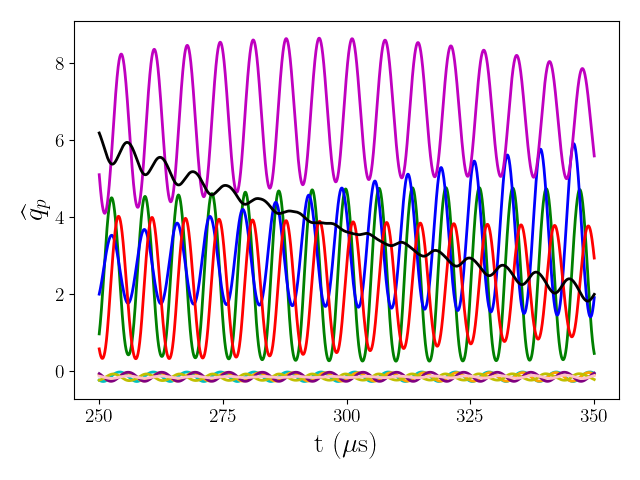
\includegraphics[width=0.6\linewidth]{Chapters/TransientFlame/Images/nonlinear/latent_vars.png}
    \caption{Encoded latent state trajectories, $f = 150$ kHz, $\numPrimModes = 10$.}
\end{figure}

\begin{figure}
    \begin{minipage}{0.49\linewidth}
        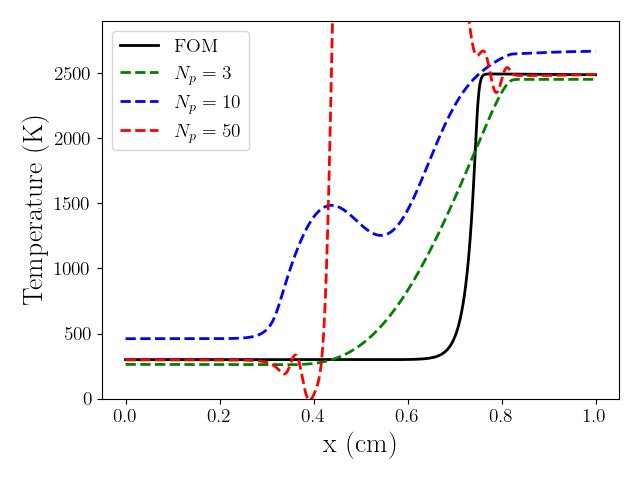
\includegraphics[width=0.99\linewidth]{Chapters/TransientFlame/Images/lstm/pod_rom_temp_snaps.png}
    \end{minipage}
    \begin{minipage}{0.49\linewidth}
        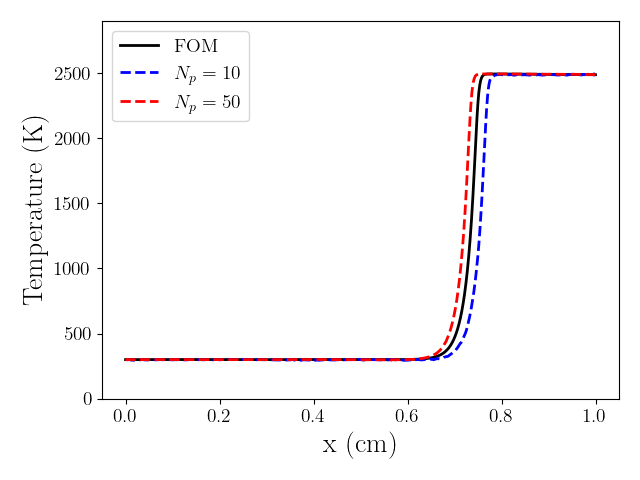
\includegraphics[width=0.99\linewidth]{Chapters/TransientFlame/Images/lstm/cae_rom_temp_snaps.png}
    \end{minipage}
    \caption{Online temperature field snapshots for LSTMs trained with POD (left) and CAE (right) trajectories, $\timeVar = XXX$, $f = 168.75$ kHz, various $\numPrimModes$.}
\end{figure}

\begin{figure}
    \begin{minipage}{0.49\linewidth}
        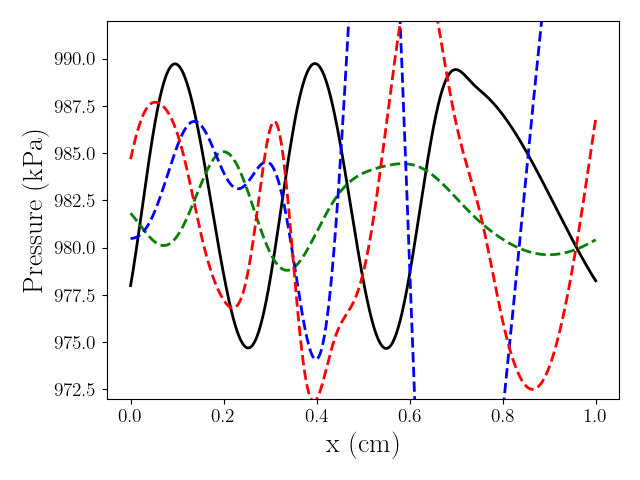
\includegraphics[width=0.99\linewidth]{Chapters/TransientFlame/Images/lstm/pod_rom_press_snaps.png}
    \end{minipage}
    \begin{minipage}{0.49\linewidth}
        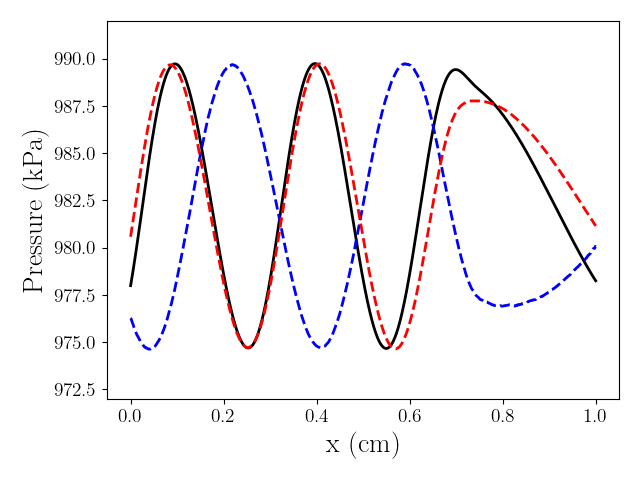
\includegraphics[width=0.99\linewidth]{Chapters/TransientFlame/Images/lstm/cae_rom_press_snaps.png}
    \end{minipage}
    \caption{Online pressure field snapshots for LSTMs trained with POD (left) and CAE (right) trajectories, $\timeVar = XXX$, $f = 168.75$ kHz, various $\numPrimModes$.}
\end{figure}

\begin{figure}
    \begin{minipage}{0.49\linewidth}
        \includegraphics[width=0.99\linewidth]{example-image-a}
        \subcaption{Upstream $f$.}
    \end{minipage}
    \begin{minipage}{0.49\linewidth}
        \includegraphics[width=0.99\linewidth]{example-image-a}
        \subcaption{Flame speed}
    \end{minipage}
    \caption{Aggregate predictions of QoIs across all forcing frequencies, all $\numPrimModes$. The best predictions for each model are marked by a bold line.}
\end{figure}